\documentclass[a4paper,10pt,oneside]{jsbook}
%
\usepackage{amsmath,amssymb,bm}
\usepackage{bm}
\usepackage[dvipdfmx]{graphicx}
\usepackage{ascmac}
\usepackage{makeidx}
\usepackage{txfonts}
\usepackage{indentfirst}
\usepackage{booktabs}
\usepackage{tabularx}
\usepackage{comment}
\AtBeginDvi{\special {pdf:tounicode EUC-UCS2}}
\usepackage[dvipdfmx, setpagesize=false, bookmarks=true, bookmarksnumbered=true]{hyperref}
\usepackage{nameref}
\usepackage{url}
\usepackage{wrapfig}

%
\makeindex
%
\newcommand{\diff}{\mathrm{d}}            %微分記号
\newcommand{\divergence}{\mathrm{div}\,}  %ダイバージェンス
\newcommand{\grad}{\mathrm{grad}\,}       %グラディエント
\newcommand{\rot}{\mathrm{rot}\,}         %ローテーション
%
\setlength{\textwidth}{\fullwidth}
\setlength{\textheight}{44\baselineskip}
\addtolength{\textheight}{\topskip}
\setlength{\voffset}{-0.6in}
%

\begin{document}

%%%%%%%%%%%%%%%%%%%%%%%%%%%%%%%%%%%%%%%%%%%%%%%%%%%%%
% 表紙
\begin{titlepage}
\noindent
独立行政法人 理化学研究所 御中
\begin{center}
	\vspace{8cm}
	{\Huge \textbf{協調ワークスペースドライバと}} \\
	\vspace{1cm}
	{\Huge \textbf{協調動作フレームワークのプロトタイプ}} \\
	\vspace{1cm}
	{\Huge \textbf{操作説明書}} \\
	\vspace{10cm}
	{\Large \textbf{2015年3月26日}} \\
	\vspace{0.5cm}
	{\Large \textbf{株式会社イマジカ デジタルスケープ}}
\end{center}
\end{titlepage}



%%%%%%%%%%%%%%%%%%%%%%%%%%%%%%%%%%%%%%%%%%%%%%%%%%%%%
% 目次
\tableofcontents

%%%%%%%%%%%%%%%%%%%%%%%%%%%%%%%%%%%%%%%%%%%%%%%%%%%%%
% 本文
%%%%%%%%%%%%%%%%%%%%%%%%%%%%%%%%%%%%%%%%%%%%%%%%%%%%%
\chapter{はじめに}
本書では協調ワークスペースドライバと協調動作フレームワークのプロトタイプの操作方法について解説します.\\

\section{動作環境とインストール}
以下の環境で動作確認を行っております.\\

\begin{tabbing}
0123\=01234567890123\=0123456789\kill
\> OS \> : Linux, Windows(Vista,7,8), MacOSX \\
\> Webブラウザ \> : Mozilla Firefox 15.x, Google Chrome 21.x, Apple Safari 6.x, Windows Internet Explorer 10.x 
\end{tabbing}

\newpage

%%%%%%%%%%%%%%%%%%%%%%%%%%%%%%%%%%%%%%%%%%%%%%%%%%%%%
% アプリケーションの展開
%%%%%%%%%%%%%%%%%%%%%%%%%%%%%%%%%%%%%%%%%%%%%%%%%%%%%
\chapter{アプリケーションの展開方法}

\subsection{Mac/Linuxの場合}
以下のコマンドを実行し解凍してください。
\begin{verbatim}
   $unzip XXXXXX.zip
\end{verbatim}


\subsection{Windowsの場合}
ダウンロードしたファイルを右クリックから、解凍を行ってください.\\
※他アーカイブ制御アプリケーションから解凍にても大丈夫です。\\


\subsection{解凍後の構成}
解凍すると、以下の構成でファイルが作成されます.\\

\begin{tabbing}
0123\=01234567890123\=0123456789\kill
\>bin        \> : 実行スクリプトフォルダ\\
\>client     \> : TDDクライアントアプリケーションフォルダ\\
\>doc        \> : ドキュメントフォルダ\\
\>redis      \> : redisアプリケーションフォルダ\\
\>server     \> : TDDサーバーアプリケーションフォルダ\\
\>package.json
\end{tabbing}

TiledDisplayDriverの起動にはbinフォルダに格納されているスクリプトを使用します.\\

\newpage

%%%%%%%%%%%%%%%%%%%%%%%%%%%%%%%%%%%%%%%%%%%%%%%%%%%%%
% インストール
%%%%%%%%%%%%%%%%%%%%%%%%%%%%%%%%%%%%%%%%%%%%%%%%%%%%%

\chapter{アプリケーションのインストール方法}

\section{インストール}

\subsection{Node.jsのインストール}
ポータルGUIの動作にはNode.jsのインストールが必要です.\\
Node.jsの公式サイト(\verb+http://nodejs.org/+)からNode.js本体をダウンロードし,インストールします.

\begin{figure}[htbp]
	\begin{center}
		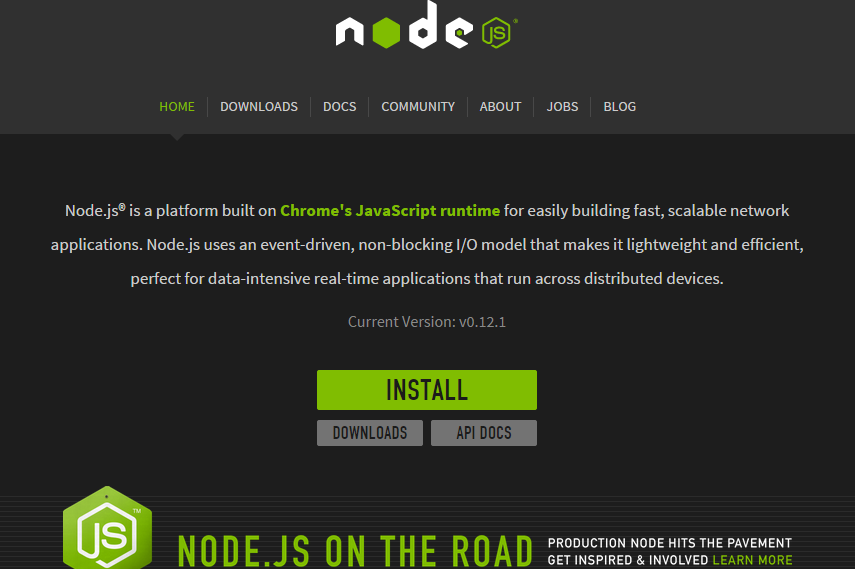
\includegraphics[width=15.5cm]{image/NodeJS.png}
	\end{center}
	\caption{node.jsのinstall画面}
	\label{fig:nodejs_home}
\end{figure}

\newpage


\subsection{Node.jsサブモジュールのインストール}
アプリケーションを展開したディレクトリに,
ポータルGUIで利用しているNode.jsの必要なサードパーティモジュールのインストールを行います.

\section{インストールスクリプトの実行}

\subsection{Mac/Linuxの場合}
bin配下の以下のシェルスクリプトを実行します.\\

\begin{verbatim}
   $cd bin
   $sh install.sh
\end{verbatim}


\subsection{Windowsの場合}
bin配下の以下のファイルを実行します.\\
\begin{verbatim}
   >cd bin
   >install.bat
\end{verbatim}

\newpage


%%%%%%%%%%%%%%%%%%%%%%%%%%%%%%%%%%%%%%%%%%%%%%%%%%%%%
% アプリケーションの起動方法
%%%%%%%%%%%%%%%%%%%%%%%%%%%%%%%%%%%%%%%%%%%%%%%%%%%%%
\chapter{アプリケーションの起動方法}


\subsection{Mac/Linuxの場合}
bin配下の以下のシェルスクリプトを実行します.\\
./run.sh

\subsection{Windowsの場合}
bin配下の以下のファイルを実行します.\\
\begin{verbatim}
   >cd bin
   >run.bat
\end{verbatim}


※
Windowsの場合、仮想メモリを0KByteにしていると、
redisが正常に起動しない場合があります.\\
その場合は一時的に仮想メモリを有効にしてご利用ください.\\

\newpage


%%%%%%%%%%%%%%%%%%%%%%%%%%%%%%%%%%%%%%%%%%%%%%%%%%%%%
% アプリケーションの起動確認
%%%%%%%%%%%%%%%%%%%%%%%%%%%%%%%%%%%%%%%%%%%%%%%%%%%%%
\section{起動確認}
起動スクリプトを実行するとポータルGUIサーバーが起動します.
\begin{verbatim}
   $sh run.sh
   (Windows版は run.bat)
\end{verbatim}

\section{コントローラへアクセス}
TDDへのアクセスは、Webブラウザのアドレス欄に「http://localhost:8080」と入力することでアクセス出来ます.\\
アクセスし、以下の画面が表示されたらインストールは完了となります。.\\

\begin{figure}[htbp]
	\begin{center}
		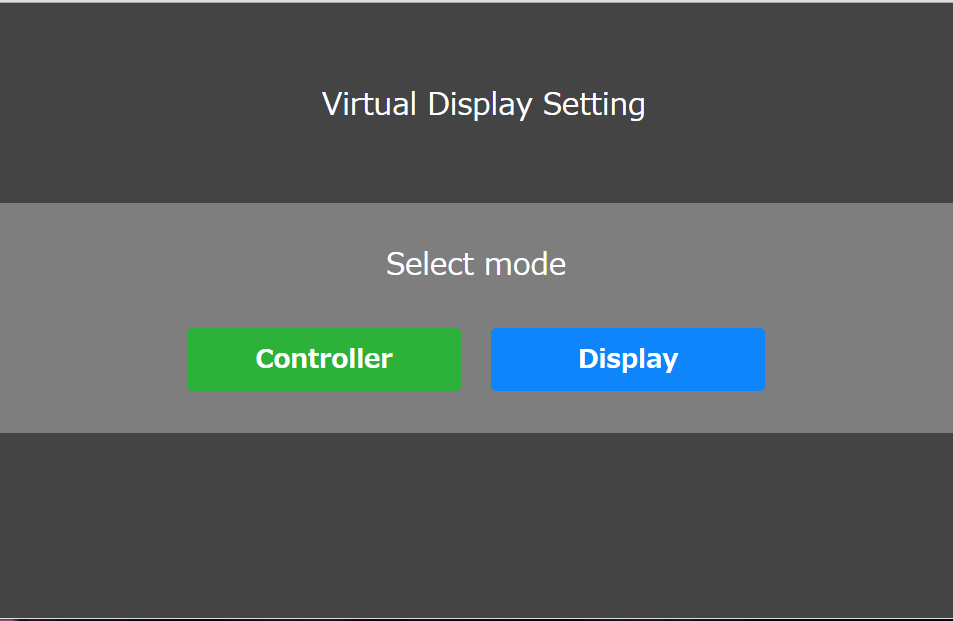
\includegraphics[width=15.5cm]{image/home.png}
	\end{center}
	\caption{insall終了後ホーム画面}
	\label{fig:home}
\end{figure}

\newpage

%%%%%%%%%%%%%%%%%%%%%%%%%%%%%%%%%%%%%%%%%%%%%%%%%%%%%
% アプリケーションの終了方法
%%%%%%%%%%%%%%%%%%%%%%%%%%%%%%%%%%%%%%%%%%%%%%%%%%%%%
\chapter{アプリケーションの終了方法}

以下2点の操作にて終了させます.\\

\subsection{1.サーバープログラムの終了}\
run.sh(bat)を起動したterminalをCTRL+Cで終了するか、
serverプログラムをkillします.\\


\subsection{2.redisの終了}
redisが起動しているterminalを終了させます.\\
また、プロセスとして起動している場合は、プロセスをpsコマンドにて見つけて
killコマンドにて終了させます.\\

\newpage

%%%%%%%%%%%%%%%%%%%%%%%%%%%%%%%%%%%%%%%%%%%%%%%%%%%%%
% TiledDisplayDriverのホーム画面
%%%%%%%%%%%%%%%%%%%%%%%%%%%%%%%%%%%%%%%%%%%%%%%%%%%%%
\chapter{TiledDisplayDriverのホーム画面}
\section{ホーム画面説明}
TDDは、以下の2つのコントローラ(Display, Controller制御)側か、Display側かを決定します.\\
TDDへのアクセスは、前述のアプリケーション起動を行った後、Webブラウザのアドレス欄に「http://localhost:8080」と入力することでアクセス出来ます.\\


\begin{figure}[htbp]
	\begin{center}
		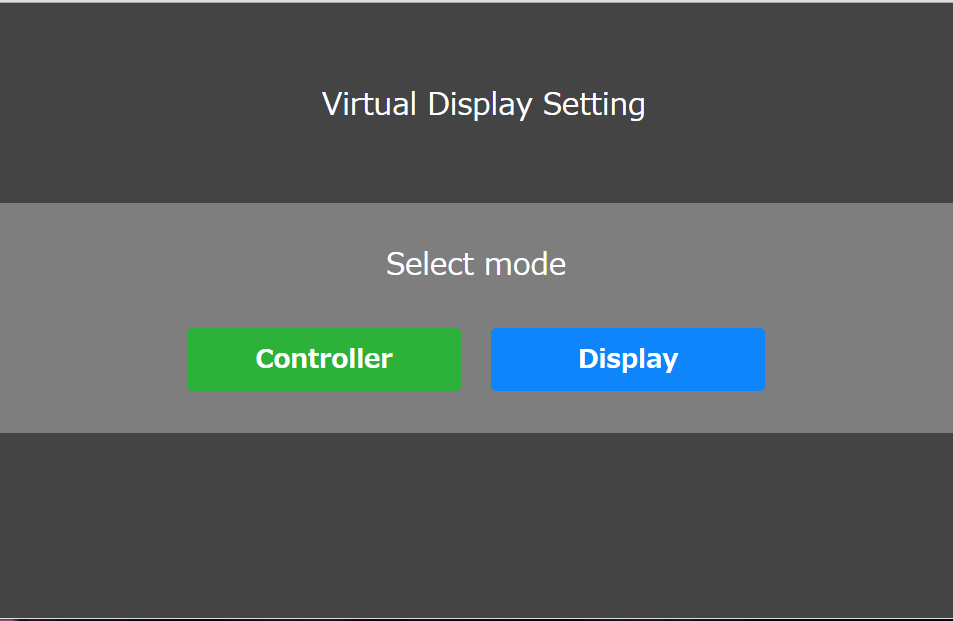
\includegraphics[width=11.5cm]{image/home.png}
	\end{center}
	\caption{ホーム画面}
	\label{fig:home}
\end{figure}


\begin{itemize}
\item Controller: コントローラ画面へと遷移します.\\
\item Display   : ディスプレイ画面へと遷移します.\\
\end{itemize}

上記の通り、アクセスしたPCを「コントローラ」として使用するか、
「ディスプレイ」として使用するかを選択することができます.\\

\newpage


%%%%%%%%%%%%%%%%%%%%%%%%%%%%%%%%%%%%%%%%%%%%%%%%%%%%%
% コントローラ画面の操作
%%%%%%%%%%%%%%%%%%%%%%%%%%%%%%%%%%%%%%%%%%%%%%%%%%%%%
\chapter{コントローラ画面の操作}
\section{概要}
コントローラは以下の通りとなっております.\\
\begin{figure}[htbp]
	\begin{center}
		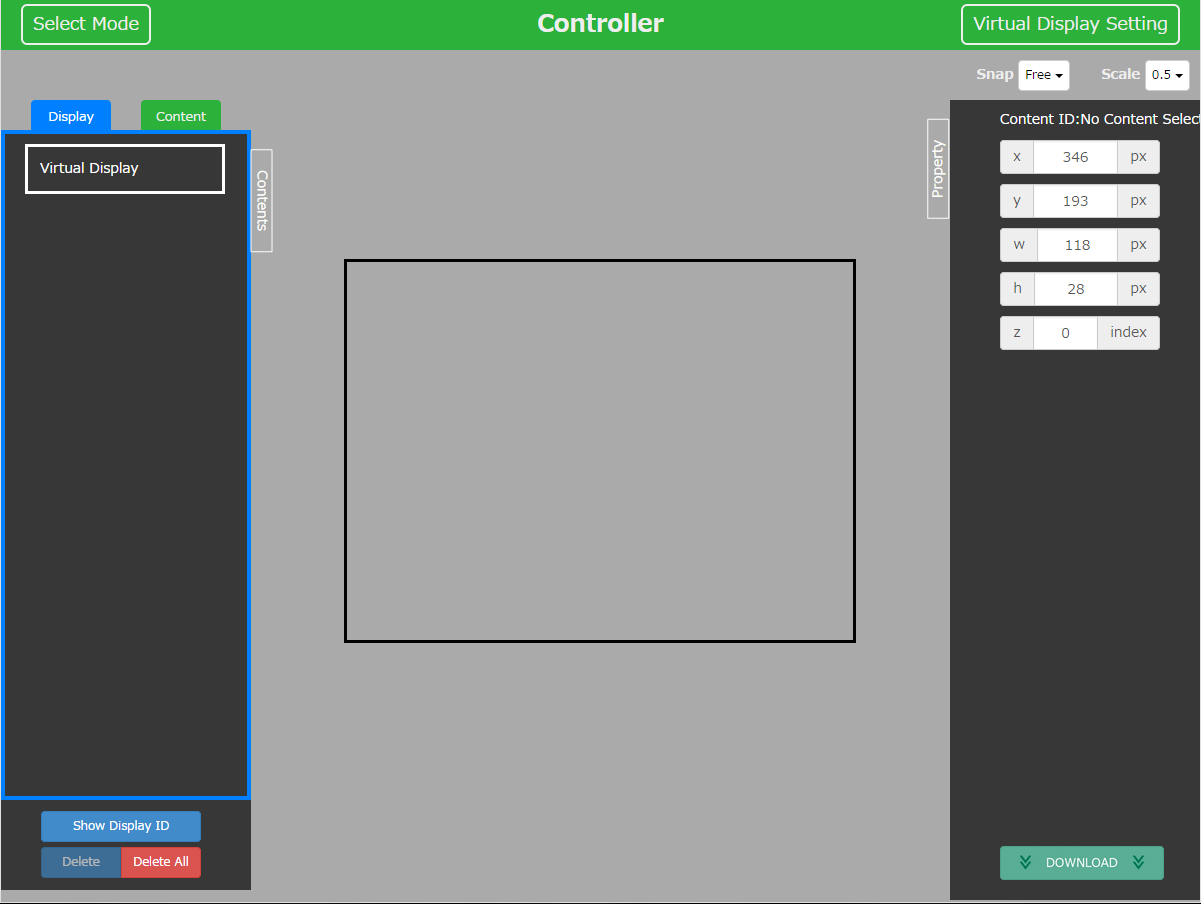
\includegraphics[width=15.5cm]{image/cont_1.PNG}
	\end{center}
	\caption{dummy}
	\label{fig:home}
\end{figure}

それぞれのタブ、ウィンドウ等、機能について解説します.\\

\newpage


%%%%%%%%%%%%%%%%%%%%%%%%%%%%%%%%%%%%%%%%%%%%%%%%%%%%%
% コントローラ画面の操作
%%%%%%%%%%%%%%%%%%%%%%%%%%%%%%%%%%%%%%%%%%%%%%%%%%%%%
\section{コントローラの操作 : VirtualDisplayScreenについて}
中央はVirtualDisplayScreenと呼ばれ、TiledDisplayServerに接続された
ディスプレイの操作、コンテンツの移動、操作、削除等を行う
汎用スペースとなっております.\\

\begin{figure}[htbp]
	\begin{center}
		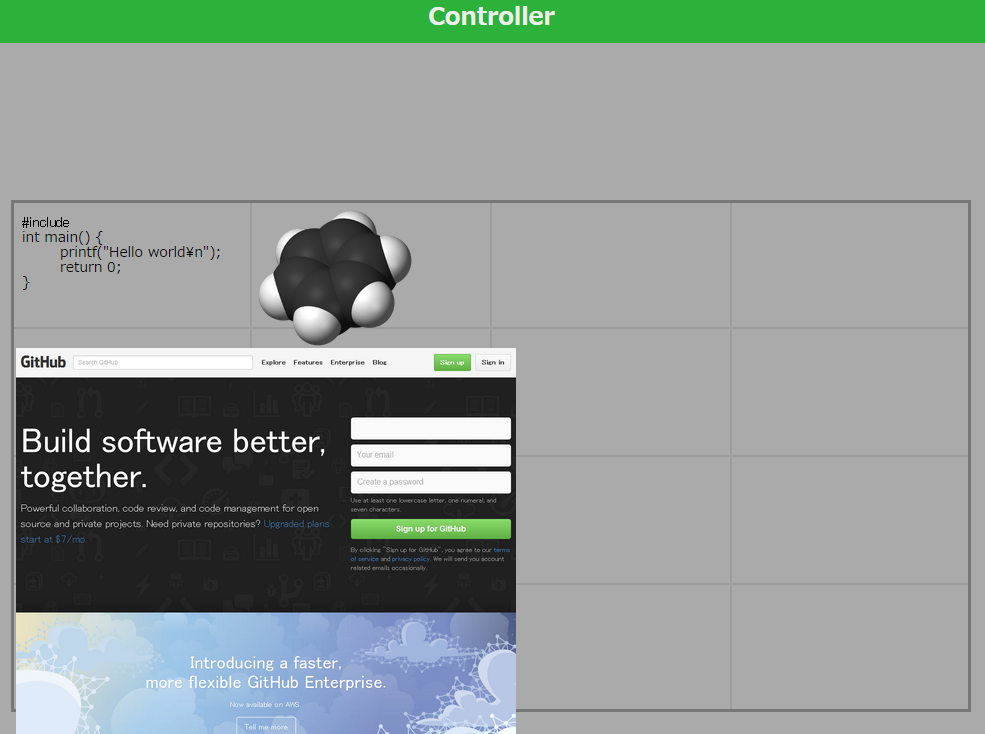
\includegraphics[width=15.5cm]{image/TDD_View.PNG}
	\end{center}
	\caption{VirtualDisplayScreenの凡例}
	\label{fig:home}
\end{figure}


\newpage


%%%%%%%%%%%%%%%%%%%%%%%%%%%%%%%%%%%%%%%%%%%%%%%%%%%%%
% コントローラ画面の操作
%%%%%%%%%%%%%%%%%%%%%%%%%%%%%%%%%%%%%%%%%%%%%%%%%%%%%
\section{コントローラの操作 : Contentsタブ(Displayタブ)}
\begin{wrapfigure}{r}{60mm}
	\begin{center}
		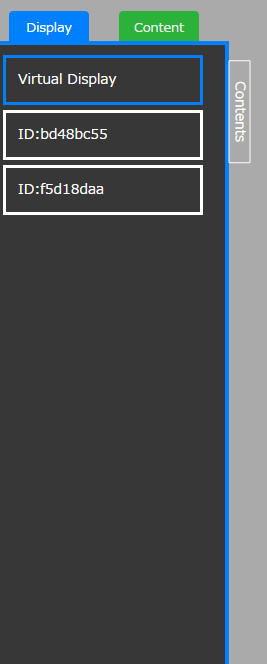
\includegraphics[width=5.5cm]{image/Display_TAB_2conn.PNG}
	\end{center}
	\caption{Contentsタブ(Displayタブ)}
	\label{fig:home}
\end{wrapfigure}

VirtualDisplayと、TDDサーバーに接続されているDisplayの一覧を表示します.\\
コントローラは、このDisplayをVirtualDisplay上に配置することができます.\\

配置したDisplay上にコンテンツを追加することによってコンテンツを共有するワークスペースを実現します.\\
Displayはマウスドラッグドロップにより、VirtualDisplaySpaceに配置することができます.\\
\\ 
右図は、2クライアントが接続された環境の例となります.


\clearpage 



%%%%%%%%%%%%%%%%%%%%%%%%%%%%%%%%%%%%%%%%%%%%%%%%%%%%%
% sub snap機能
%%%%%%%%%%%%%%%%%%%%%%%%%%%%%%%%%%%%%%%%%%%%%%%%%%%%%
\subsection{snap機能}
Displayを正確に区画に配置するための機能として「snap機能」があります.\\
画面右側の以下のボタンとなります.\\

\begin{tabbing}
0123\=01234567890123\=0123456789\kill
\>Free    \> : 自由配置となります.\\
\>Display \> : 分割した区画に沿ってDisplayがスナップするようになります.
\end{tabbing}

以下にsnap機能を用いて配置する凡例を示します。.\\

\begin{figure}[htbp]
	\begin{center}
		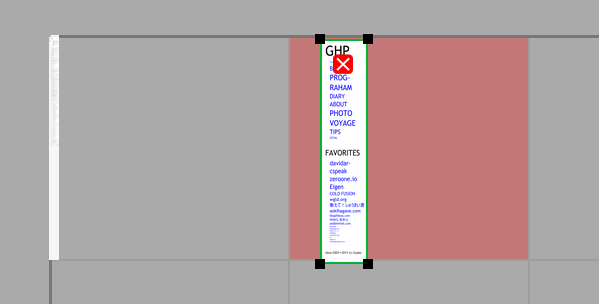
\includegraphics[width=15.5cm]{image/Snap1.png}
	\end{center}
	\caption{Snap機能ドラッグ時凡例}
	\label{fig:}
\end{figure}


またVirtualDisplaySpaceの拡大縮小オプションとして、Scale機能があります。図\ref{fig:scale}のボタンとなります.\\

\begin{figure}[htbp]
	\begin{center}
		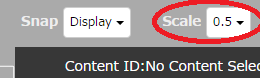
\includegraphics[width=7.5cm]{image/MIGIUE_Scale.PNG}
	\end{center}
	\caption{dummy}
	\label{fig:scale}
\end{figure}

デフォルトは0.5となっております.\\



\clearpage 


%%%%%%%%%%%%%%%%%%%%%%%%%%%%%%%%%%%%%%%%%%%%%%%%%%%%%
% sub Show Display IDボタン
%%%%%%%%%%%%%%%%%%%%%%%%%%%%%%%%%%%%%%%%%%%%%%%%%%%%%
\subsection{Show Display IDボタン}
接続されたDisplayのIDを各接続されたDisplay上に表示し、識別できるようにします.\\
尚、IDは、接続された端末固有であり、1端末につき1IDが割り当てられます.\\
\begin{figure}[htbp]
	\begin{center}
		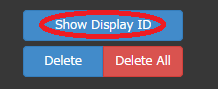
\includegraphics[width=7.5cm]{image/3Button1.PNG}
	\end{center}
	\caption{Show Display ID}
	\label{fig:home}
\end{figure}


%%%%%%%%%%%%%%%%%%%%%%%%%%%%%%%%%%%%%%%%%%%%%%%%%%%%%
% sub Deleteボタン
%%%%%%%%%%%%%%%%%%%%%%%%%%%%%%%%%%%%%%%%%%%%%%%%%%%%%
\subsection{Delete}
選択したDisplayを削除(TDDサーバーから切断)します.\\
\begin{figure}[htbp]
	\begin{center}
		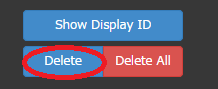
\includegraphics[width=7.5cm]{image/3Button2.PNG}
	\end{center}
	\caption{dummy}
	\label{fig:home}
\end{figure}

※尚、VirtualDisplayは削除することはできません.\\



%%%%%%%%%%%%%%%%%%%%%%%%%%%%%%%%%%%%%%%%%%%%%%%%%%%%%
% sub DeleteAllボタン
%%%%%%%%%%%%%%%%%%%%%%%%%%%%%%%%%%%%%%%%%%%%%%%%%%%%%
\subsection{DeleteAllボタン}
接続されているDisplayすべてを削除(TDDサーバーから切断)します.\\

\begin{figure}[htbp]
	\begin{center}
		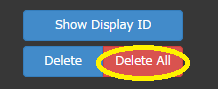
\includegraphics[width=7.5cm]{image/3Button3.PNG}
	\end{center}
	\caption{dummy}
	\label{fig:home}
\end{figure}

\newpage


%%%%%%%%%%%%%%%%%%%%%%%%%%%%%%%%%%%%%%%%%%%%%%%%%%%%%
% sub コントローラの操作
%%%%%%%%%%%%%%%%%%%%%%%%%%%%%%%%%%%%%%%%%%%%%%%%%%%%%
\section{コントローラの操作 : 左(contentsタブ)}
各ボタンの機能は以下の通りとなります.\\

\subsection{Addボタン}
コンテンツの追加を行います.\\
押下することで、AddContentウィンドウを開きます



%%%%%%%%%%%%%%%%%%%%%%%%%%%%%%%%%%%%%%%%%%%%%%%%%%%%%
% sub テキストファイルの追加
%%%%%%%%%%%%%%%%%%%%%%%%%%%%%%%%%%%%%%%%%%%%%%%%%%%%%
\subsection{テキストファイルの追加}
Contentポップアップからテキストファイルをコンテンツに追加します.\\
以下追加例となります.\\

\begin{figure}[htbp]
	\begin{center}
		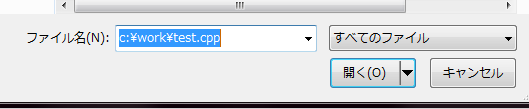
\includegraphics[width=11.5cm]{image/AddContent_TextFile_Select.png}
	\end{center}
	\caption{テキストファイルを選択}
	\label{fig:home}
\end{figure}


\begin{figure}[htbp]
	\begin{center}
		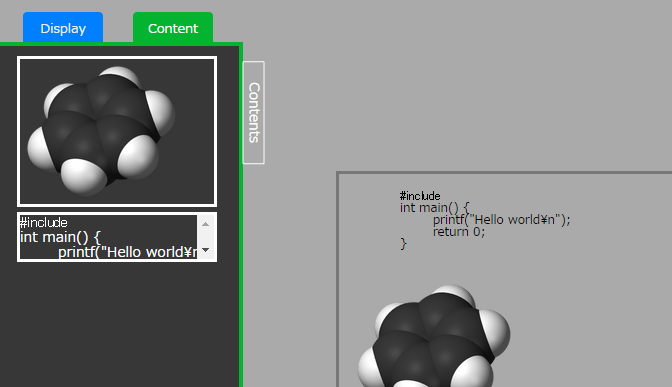
\includegraphics[width=15.5cm]{image/AddContent_TextFile_View.png}
	\end{center}
	\caption{テキストファイルのVirtualScreenへの追加}
	\label{fig:home}
\end{figure}

\newpage



%%%%%%%%%%%%%%%%%%%%%%%%%%%%%%%%%%%%%%%%%%%%%%%%%%%%%
% sub URLの送信
%%%%%%%%%%%%%%%%%%%%%%%%%%%%%%%%%%%%%%%%%%%%%%%%%%%%%
\subsection{URLの送信}
Contentポップアップから入力されたURLのサイトの画像をコンテンツに追加します.\\
以下例となります.\\
\begin{figure}[htbp]
	\begin{center}
		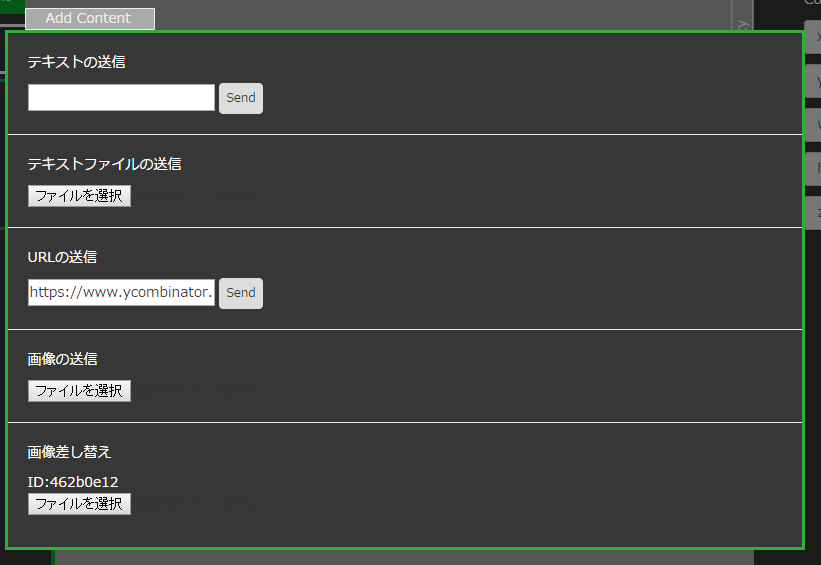
\includegraphics[width=12.5cm]{image/AddContent_URL.PNG}

	\end{center}
	\caption{dummy}
	\label{fig:home}
\end{figure}

追加すると以下の通りとなります.\\


\begin{figure}[htbp]
	\begin{center}
		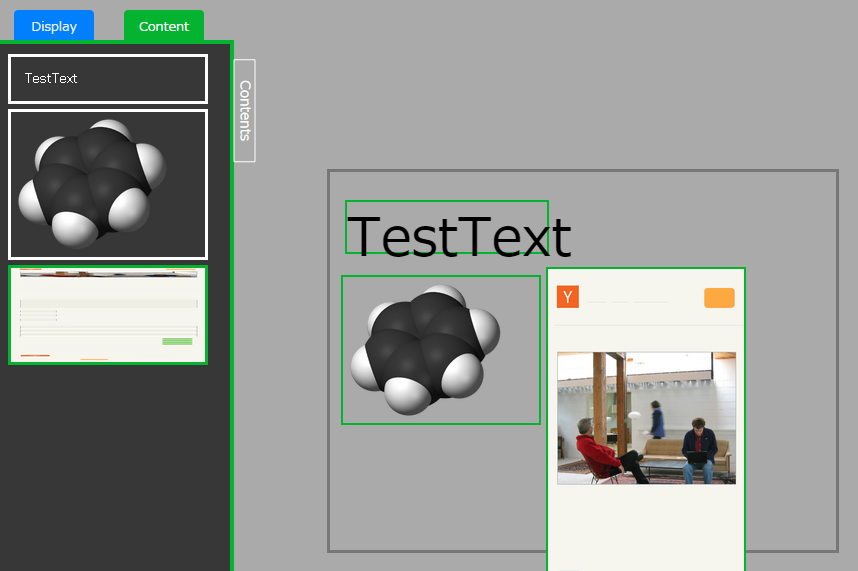
\includegraphics[width=12.5cm]{image/AddContent_URL_View.PNG}
	\end{center}
	\caption{dummy}
	\label{fig:home}
\end{figure}

\newpage





%%%%%%%%%%%%%%%%%%%%%%%%%%%%%%%%%%%%%%%%%%%%%%%%%%%%%
% sub 画像の送信
%%%%%%%%%%%%%%%%%%%%%%%%%%%%%%%%%%%%%%%%%%%%%%%%%%%%%
\subsection{画像の送信}
Contentポップアップから任意の画像ファイルをコンテンツに追加します.\\
対応している画像フォーマットは以下の通りです.\\

\begin{itemize}
\item PNGフォーマット形式.
\item JPEGフォーマット形式.
\end{itemize}

以下は表示例となります.\\
\begin{figure}[htbp]
	\begin{center}
		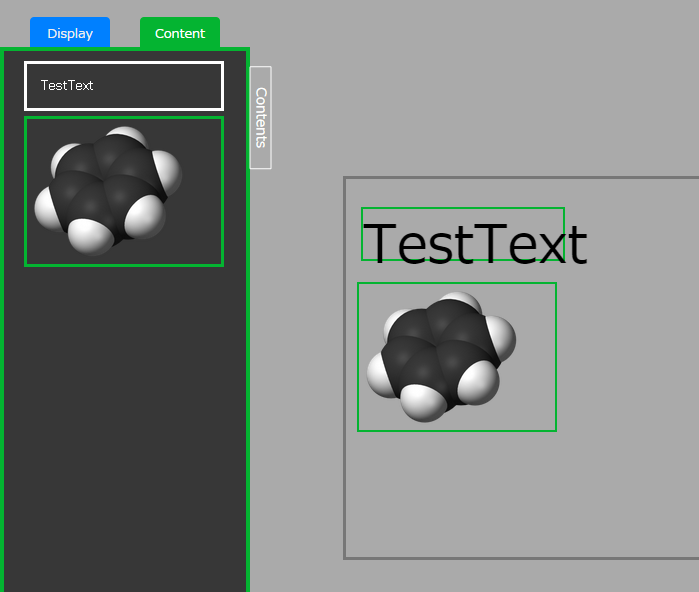
\includegraphics[width=11.5cm]{image/AddContent_Picture_View.PNG}
	\end{center}
	\caption{画像の追加凡例}
	\label{fig:home}
\end{figure}



\newpage

%%%%%%%%%%%%%%%%%%%%%%%%%%%%%%%%%%%%%%%%%%%%%%%%%%%%%
% sub 画像の差し替え
%%%%%%%%%%%%%%%%%%%%%%%%%%%%%%%%%%%%%%%%%%%%%%%%%%%%%
\subsection{画像の差し替え}
contentsタブにて選択している画像の差し替えを行います.\\
差し替え例を以下に示します.\\
★画面のスクリーンショット
\begin{figure}[htbp]
	\begin{center}
		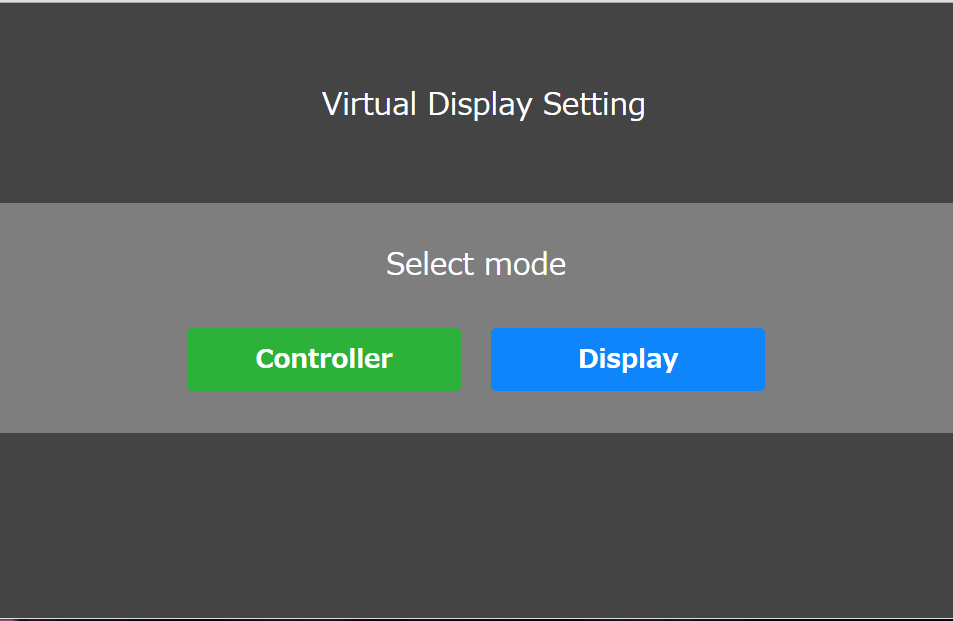
\includegraphics[width=11.5cm]{image/home.png}
	\end{center}
	\caption{画像の差し替え凡例}
	\label{fig:home}
\end{figure}




\clearpage 

%%%%%%%%%%%%%%%%%%%%%%%%%%%%%%%%%%%%%%%%%%%%%%%%%%%%%
% プロパティタブ
%%%%%%%%%%%%%%%%%%%%%%%%%%%%%%%%%%%%%%%%%%%%%%%%%%%%%
\chapter{コントローラの操作 : propartyウィンドウ }
\begin{wrapfigure}{r}{60mm}
	\begin{center}
		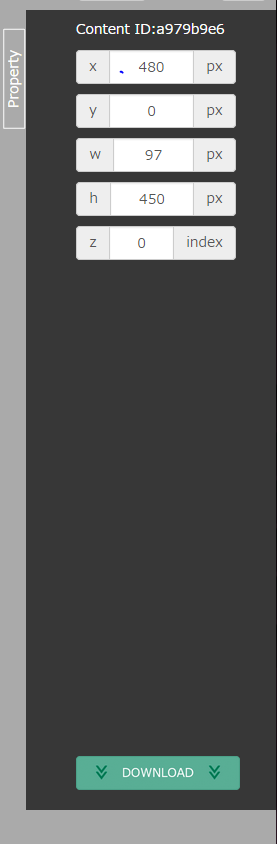
\includegraphics[width=5.5cm]{image/Prop_Down.PNG}
	\end{center}
	\caption{propartyウィンドウ}
	\label{fig:propall}
\end{wrapfigure}

propartyウィンドウは選択されたコンテンツ、Display、ContentsのID、
およびそれぞれのpropartyを表示します.\\

propartyは以下の通りID以外を編集し、座標、表示全面の優先順位 Zindex を
指定することができます.\\


また、選択されたContentsはpropartyウィンドウ左下のダウンロードボタンから
ダウンロードすることができます.\\


\clearpage 



%%%%%%%%%%%%%%%%%%%%%%%%%%%%%%%%%%%%%%%%%%%%%%%%%%%%%
% コントローラの操作 : 上記操作
%%%%%%%%%%%%%%%%%%%%%%%%%%%%%%%%%%%%%%%%%%%%%%%%%%%%%
\chapter{コントローラの操作 : 上部表示領域}
\subsection{Controllerボタン}
Displayウィンドウを表示します.\\
現状は押下しても特に意味を持ちません.\\

\subsection{Displayボタン}
Displayウィンドウを新しいタブで表示します.\\

\begin{figure}[htbp]
	\begin{center}
		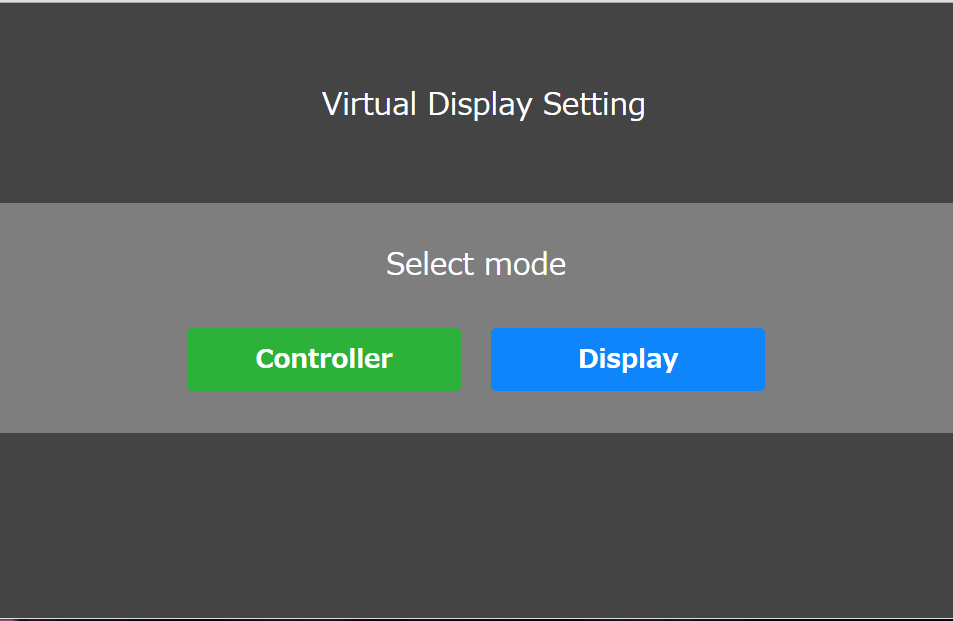
\includegraphics[width=11.5cm]{image/home.png}
	\end{center}
	\caption{ホーム画面}
	\label{fig:home}
\end{figure}


\subsection{Virtual Display Settingボタン}
Displayタブに操作をフォーカスします.\\

\begin{figure}[htbp]
	\begin{center}
		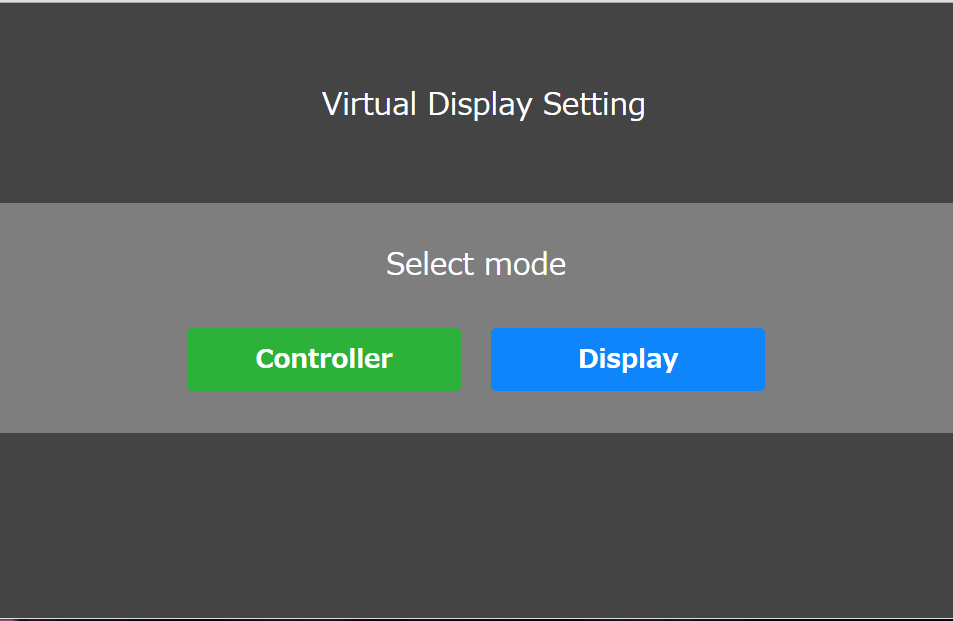
\includegraphics[width=11.5cm]{image/home.png}
	\end{center}
	\caption{ホーム画面}
	\label{fig:home}
\end{figure}

\end{document}
